\documentclass{article}
\usepackage{CJKutf8}
\usepackage{graphicx}
\usepackage{amsthm}
\let\proof\relax \let\endproof\relax % 避免 math_blog 重复定义 proof 报错
\usepackage{math_blog}
\usepackage{amsmath}
\usepackage{amssymb}
\usepackage{appendix}
\usepackage[normalem]{ulem}
\usepackage[thicklines]{cancel}
\usepackage{tikz}
\usetikzlibrary{positioning,arrows.meta}
\usepackage{pgfplots}

% Defensive: resolve possible \proof / theorem-env conflicts with math_blog
\makeatletter
\@ifundefined{proof}{}{\let\proof\@undefined \let\endproof\@undefined}
\@ifundefined{theorem}{\newtheorem{theorem}{Theorem}[section]}{}
\@ifundefined{lemma}{\newtheorem{lemma}[theorem]{Lemma}}{}
\@ifundefined{definition}{\newtheorem{definition}[theorem]{Definition}}{}
\@ifundefined{proposition}{\newtheorem{proposition}[theorem]{Proposition}}{}
\@ifundefined{corollary}{\newtheorem{corollary}[theorem]{Corollary}}{}
\@ifundefined{remark}{\newtheorem*{remark}{Remark}}{}
\@ifundefined{example}{\newtheorem*{example}{Example}}{}
\makeatother
\newenvironment{proof}[1][证明]{%
  \par\smallskip\noindent\textit{\textbf{#1.}}\quad\ignorespaces
}{%
  \hfill$\square$\par\smallskip
}

% 中文环境名（与 theorem 共用计数器）
\theoremstyle{plain}
\newtheorem{zhtheorem}[theorem]{定理}
\newtheorem{zhlemma}[theorem]{引理}
\newtheorem{zhcorollary}[theorem]{推论}
\theoremstyle{definition}
\newtheorem{zhdefinition}[theorem]{定义}
\newtheorem{zhexample}[theorem]{例}
\theoremstyle{remark}
\newtheorem*{zhremark}{注}
\let\theorem\zhtheorem \let\endtheorem\endzhtheorem
\let\lemma\zhlemma \let\endlemma\endzhlemma
\let\corollary\zhcorollary \let\endcorollary\endzhcorollary
\let\definition\zhdefinition \let\enddefinition\endzhdefinition
\let\example\zhexample \let\endexample\endzhexample
\let\remark\zhremark \let\endremark\endzhremark
\renewcommand{\figurename}{图}
\renewcommand{\tablename}{表}
\renewcommand{\refname}{参考文献}

\title{[SDE IV] 倒向随机微分方程与非线性 Feynman--Kac 公式}
\author{Anqiao Ouyang, Xuecheng Liu}
\date{May 27, 2026}

\newcommand{\Title}{倒向随机微分方程与非线性 Feynman--Kac 公式}
% 标题较长：放到页眉右侧，避免与作者名重叠
\fancyhead[C]{}
\fancyhead[R]{\small\textit{\Title}}
\newcommand{\Column}{Stochastic Differential Equations IV}
\newcommand{\Author}{Anqiao Ouyang, Xuecheng Liu}

% Math shortcuts
\newcommand{\E}{\mathbb{E}}
\newcommand{\Prob}{\mathbb{P}}
\newcommand{\R}{\mathbb{R}}
\newcommand{\F}{\mathcal{F}}
\newcommand{\Lc}{\mathcal{L}}
\newcommand{\Sc}{\mathcal{S}}
\newcommand{\Hc}{\mathcal{H}}

\begin{document}
\begin{CJK*}{UTF8}{gbsn}

\maketitle

\section{引言}

本专栏前三篇文章主要围绕前向随机微分方程展开。在 [SDE~I] 我们构造了布朗运动，并铺设了相关的测度论基础；在 [SDE~II] 我们发展了 It\^o 积分以及随机分析的链式法则；在 [SDE~III] 我们证明了前向 SDE 的解的存在唯一性，并通过 \textbf{Feynman--Kac 公式}跨入到 PDE 的世界：对线性抛物型问题
\[
  \partial_t u + \Lc u = 0, \qquad u(T,x) = g(x),
\]
其中 $\Lc$ 是 $X$ 的无穷小生成元，解具有概率表示
\[
  u(t,x) = \E\big[g(X_T) \,\big|\, X_t = x\big].
\]

一个自然的问题是：如果在 PDE 中加入一个非线性源项，会发生什么？
\[
  \partial_t u + \Lc u + f\!\big(t, x, u, \sigma^{\top}\nabla u\big) = 0, \qquad u(T, x) = g(x).
\]
线性 Feynman--Kac 中的期望在固定时刻 $T$ 取，被积函数里并不含 $u$ 或 $\nabla u$。要把它们纳入，需要一个能让信息\emph{沿时间反向传递}的表示，把 $X$ 在整个 $[t, T]$ 上的路径都纳入条件。完成这项工作的对象正是\textbf{倒向随机微分方程}（backward stochastic differential equation，BSDE）。

形式上，BSDE 是一条从终端条件 $Y_T = \xi$ 倒回 $0$ 时刻的“SDE”：
\[
  -dY_t = f(t, Y_t, Z_t)\,dt - Z_t\, dB_t, \qquad Y_T = \xi.
\]
未知量是一对过程 $(Y_t, Z_t)$：$Y$ 是实值过程，$Z$ 是针对布朗运动的被积函数。我们在 \S2 会看到，$Z$ 并非额外的数据选择，而是适应性条件（通过鞅表示定理）强加给我们的。当 $\xi = g(X_T)$、且 $f$ 以 Markov 方式依赖 $(t, X_t, Y_t, Z_t)$ 时，BSDE 恰好求解上述半线性 PDE，并有对应关系
\[
  Y_t = u(t, X_t), \qquad Z_t = \sigma^{\top}(t, X_t)\, \nabla u(t, X_t).
\]
这就是 Pardoux 与 Peng 的\textbf{非线性 Feynman--Kac 公式}。

该理论由 Pardoux 与 Peng 于 1990 年提出\cite{pp1990}，如今已深植于随机控制、数理金融，以及近年的深度学习 PDE 求解器中。本文将：

\begin{itemize}
  \item 精确定义 BSDE，并说明为什么 $(Y, Z)$ 这一对才是正确的未知量（\S2）；
  \item 在 Lipschitz 条件下证明 Pardoux--Peng 的存在唯一性定理（\S3）；
  \item 建立比较定理，并观察它如何反映定价的无套利结构（\S4）；
  \item 为 Markov 型 BSDE 证明非线性 Feynman--Kac 公式，与 [SDE~III] 中的线性版本并列对比（\S5）；
  \item 将这套机制应用于随机最优控制（HJB），并概述 Deep BSDE 数值方法（\S6）；
  \item 以前向倒向耦合、平均场 BSDE、反射型 BSDE 与粗糙路径收尾（\S7）。
\end{itemize}

\paragraph{标准记号。} 我们在带流的概率空间 $(\Omega, \F, (\F_t)_{0 \le t \le T}, \Prob)$ 上工作，其上有 $d$ 维布朗运动 $B = (B_t)_{0 \le t \le T}$，$(\F_t)$ 为 $B$ 的扩充流，固定时间视域 $T > 0$。向量按列排列，$\sigma^{\top}$ 表示矩阵转置，$|\cdot|$ 是欧氏范数。“适应的”指 $(\F_t)$-适应，“可预测的”指 $(\F_t)$-可预测。$K$ 为一般性常数，其数值可能逐行变动。

\section{BSDE 的定义与 \texorpdfstring{$Z$}{Z} 的角色}

\subsection{为什么需要一对？}

设想我们以最朴素的方式定义倒向 SDE：取终端条件 $\xi \in L^2(\F_T)$ 和驱动函数 $f(t, y)$，寻找 $(\F_t)$-适应的过程 $Y$ 满足
\[
  Y_T = \xi, \qquad -dY_t = f(t, Y_t)\,dt.
\]
这只是一个逐轨道从 $T$ 倒推的 ODE。问题出在适应性：$Y_T = \xi$ 是 $\F_T$-可测的，因此由 ODE 从 $T$ 倒推回去的 $Y_t$ 会继承 $\xi$ 的所有信息，这在任何更早的时刻 $t < T$ 都违反 $\F_t$-可测性。换句话说，知道 $Y_t$ 就能预测 $\xi$。

补救方法是允许一个\textbf{鞅修正项}。根据鞅表示定理（如 \cite{revuz-yor}, Ch.~V），每个满足 $M_0 = \E[\xi]$ 的平方可积布朗鞅 $M$ 都存在唯一的可预测被积函数 $Z \in \Hc^2$ 使得
\[
  M_t = M_0 + \int_0^t Z_s\, dB_s.
\]
取 $M_t := \E[\xi \mid \F_t]$，就得到那个“承载”截至时刻 $t$ 为止有关 $\xi$ 之信息的 $Z$。BSDE 就是把确定性驱动 $f$ 与这个布朗修正项 $Z\, dB$ 结合起来的积分等式。

\begin{definition}[BSDE 的解]\label{def:bsde}
设 $\xi \in L^2(\F_T; \R)$，$f : [0,T] \times \Omega \times \R \times \R^d \to \R$ 循序可测。称一对过程 $(Y, Z)$（其中 $Y$ 连续、实值、$(\F_t)$-适应，$Z$ 为 $(\F_t)$-可预测且取值于 $\R^d$）为 BSDE $(\xi, f)$ 的\emph{解}，若
\begin{equation}\label{eq:bsde}
  Y_t = \xi + \int_t^T f(s, Y_s, Z_s)\,ds - \int_t^T Z_s\, dB_s, \qquad t \in [0, T],
\end{equation}
$\Prob$-a.s.\ 成立，且
\[
  \E\!\Big[\sup_{0 \le t \le T}|Y_t|^2\Big] < \infty, \qquad \E\!\int_0^T |Z_s|^2\,ds < \infty.
\]
\end{definition}

我们给解空间命名：
\[
  \Sc^2 := \Big\{Y \text{ 适应、连续} : \|Y\|_{\Sc^2}^2 := \E\!\big[\sup_t |Y_t|^2\big] < \infty\Big\},
\]
\[
  \Hc^2 := \Big\{Z \text{ 可预测} : \|Z\|_{\Hc^2}^2 := \E\!\int_0^T |Z_s|^2\,ds < \infty\Big\}.
\]
$\Sc^2$ 在上述范数下是 Banach 空间，$\Hc^2$ 是 Hilbert 空间。方程 \eqref{eq:bsde} 应在 $\Sc^2 \times \Hc^2$ 中理解。

\begin{remark}
对 \eqref{eq:bsde} 求微分，得到微分形式
\[
  -dY_t = f(t, Y_t, Z_t)\,dt - Z_t\, dB_t, \qquad Y_T = \xi.
\]
$dY$ 前的负号只是记号约定：它表明时间从 $T$ 倒推。有些作者把它吸收进驱动函数，写成 $\widetilde{f} = -f$。
\end{remark}

\begin{figure}[htbp]
\centering
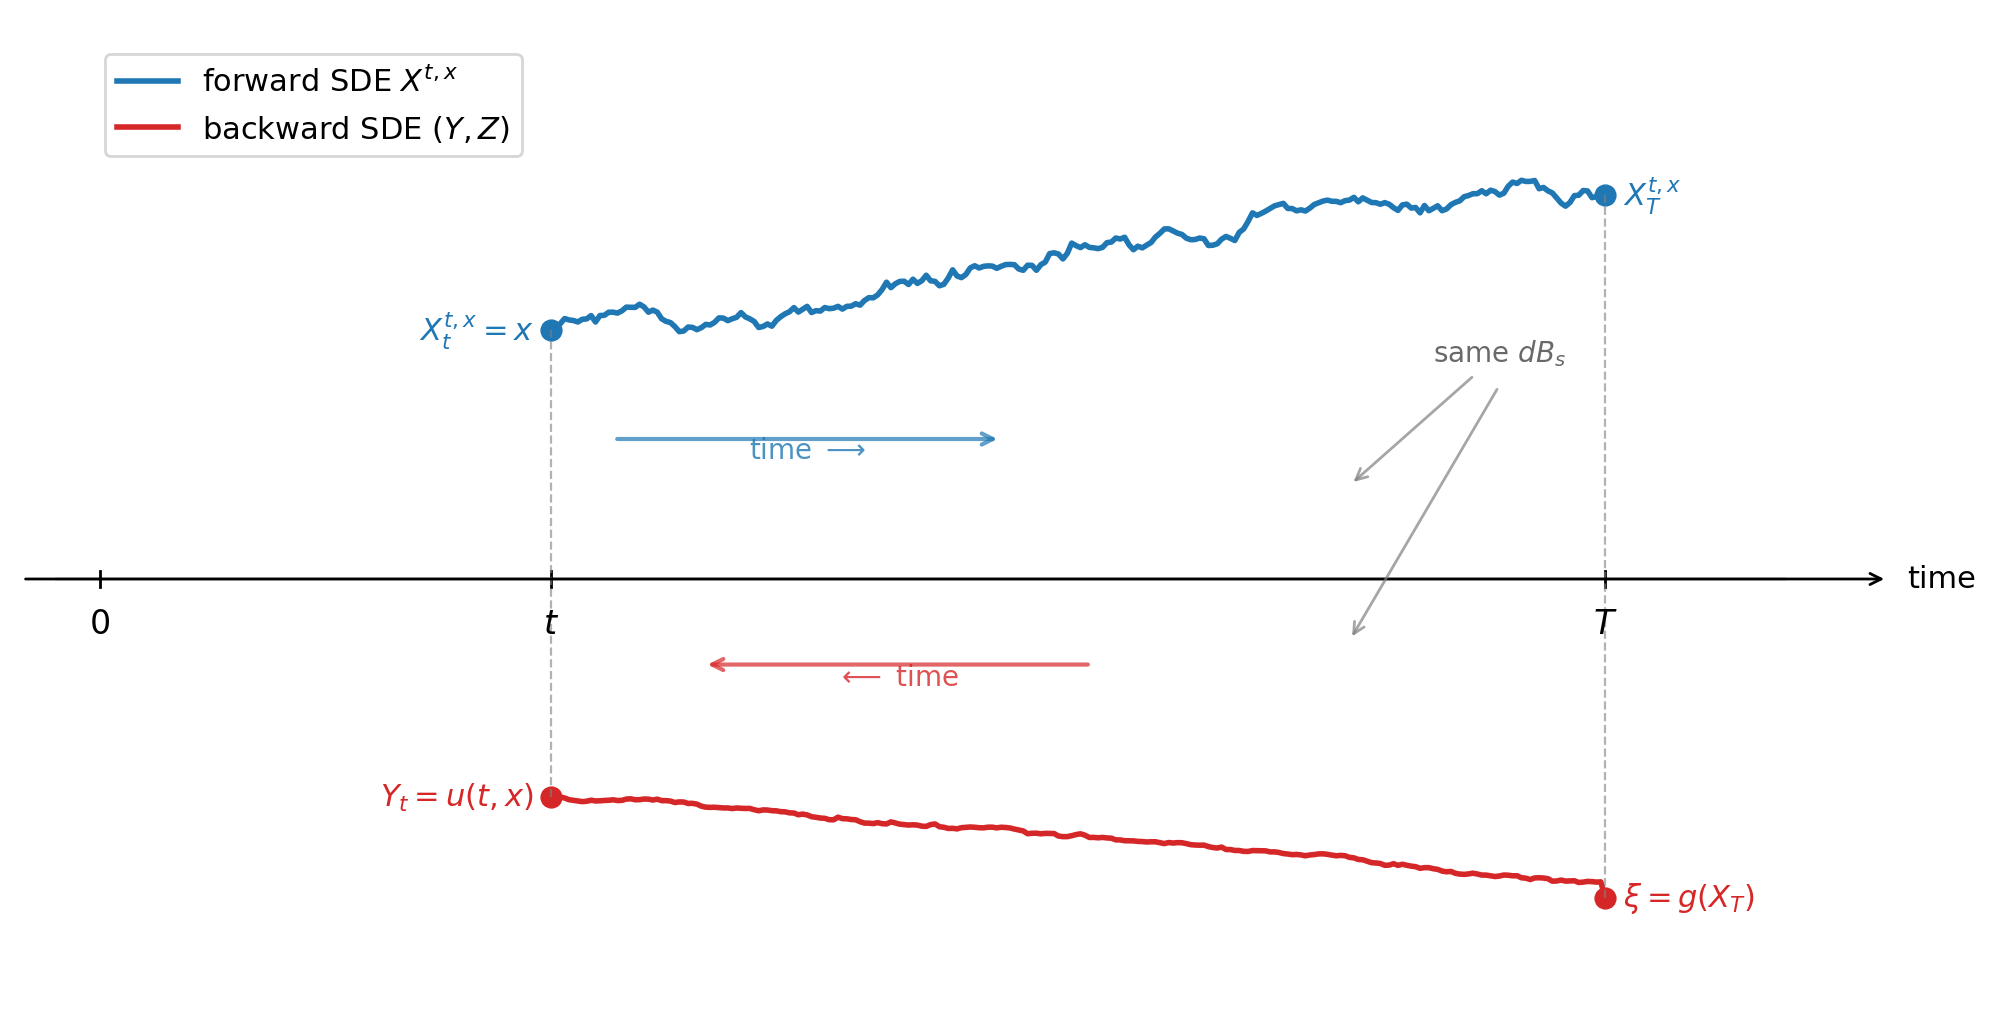
\includegraphics[width=0.95\linewidth]{figures/fig1_fwd_bwd.png}
\caption{非线性 Feynman--Kac 公式背后的前向与倒向图像。扩散 $X^{t,x}$ 在时刻 $t$ 从 $x$ 出发，\emph{正向}演化到随机的终端值 $X_T$；接着终端收益 $\xi = g(X_T)$ 由 BSDE \emph{倒向}传递，生成 $Y_t = u(t,x)$。两个过程被 $[t,T]$ 上同一组布朗增量 $dB_s$ 驱动：前向方程通过扩散系数 $\sigma$，倒向方程通过被积函数 $Z$。适应性要求 $Y_t$ 只能是截至 $t$ 为止的历史的函数，这正是 $Z$ 不可或缺的原因。}
\label{fig:fwd-bwd}
\end{figure}

\subsection{两个热身例子}

\begin{example}[$f \equiv 0$：伪装的线性 Feynman--Kac]
BSDE $(\xi, 0)$ 化为 $Y_t = \xi - \int_t^T Z_s\,dB_s$。取条件期望，
\[
  Y_t = \E[\xi \mid \F_t],
\]
而 $Z$ 是 $M_t = \E[\xi \mid \F_t]$ 的鞅表示中的被积函数。零驱动的 BSDE 正是线性 Feynman--Kac 公式。专门取 $\xi = g(X_T)$ 即可还原 [SDE~III, 定理~4.1]。
\end{example}

\begin{example}[线性驱动与显式解]
对于 $f(t, y, z) = \alpha_t\, y + \beta_t \cdot z + \gamma_t$（系数有界、适应），定义折现因子与变测度因子
\[
  \Gamma_t := \exp\!\Big(\int_0^t \alpha_s\, ds\Big), \qquad \frac{d\Prob^\beta}{d\Prob}\bigg|_{\F_T} := \exp\!\Big(\int_0^T \beta_s\, dB_s - \tfrac12\!\int_0^T |\beta_s|^2 ds\Big).
\]
则
\[
  \Gamma_t\, Y_t = \E^{\Prob^\beta}\!\Big[ \Gamma_T\, \xi + \int_t^T \Gamma_s\, \gamma_s\, ds \,\Big|\, \F_t\Big].
\]
这个公式正是 BSDE 版本的“常数变易法”，后面证明比较定理时会用到。
\end{example}

\section{存在性与唯一性}

BSDE 理论的基石结果如下。

\begin{theorem}[Pardoux--Peng, 1990]\label{thm:pp}
假设
\begin{enumerate}
  \item[(i)] $\xi \in L^2(\F_T)$；
  \item[(ii)] $(t, \omega) \mapsto f(t, \omega, 0, 0)$ 属于 $\Hc^2$；
  \item[(iii)] $f$ 对 $(y, z)$ 一致 Lipschitz，即存在 $K \ge 0$ 使得
    \[
      |f(t, \omega, y, z) - f(t, \omega, y', z')| \le K\big(|y - y'| + |z - z'|\big)
    \]
    对 $dt \otimes d\Prob$-几乎所有 $(t,\omega)$ 成立。
\end{enumerate}
则 BSDE \eqref{eq:bsde} 在 $\Sc^2 \times \Hc^2$ 中有唯一解 $(Y, Z)$。
\end{theorem}

证明的精神类似于前向 SDE 的 Picard 迭代（[SDE~III, \S2]），但引入一个新元素：压缩发生在带\emph{指数权重}的范数下，权重恰好吸收 Lipschitz 常数。

\subsection{先验估计}

\begin{lemma}[先验界]\label{lem:apriori}
若 $(Y, Z) \in \Sc^2 \times \Hc^2$ 解 \eqref{eq:bsde}，则对任意 $\beta > 2K + 2K^2$，
\[
  \E\!\int_0^T e^{\beta s}\big(|Y_s|^2 + |Z_s|^2\big)\,ds \le C \!\left( \E\big[ e^{\beta T}|\xi|^2 \big] + \E\!\int_0^T e^{\beta s}|f(s, 0, 0)|^2\, ds \right),
\]
其中常数 $C$ 仅依赖于 $K$ 与 $\beta$。
\end{lemma}

\begin{proof}[证明（纲要）]
对 $\varphi_t := e^{\beta t} |Y_t|^2$ 应用 It\^o 公式：
\[
  d\varphi_t = \beta e^{\beta t}|Y_t|^2\,dt + 2 e^{\beta t} Y_t\,dY_t + e^{\beta t} |Z_t|^2\,dt.
\]
代入 $dY_t = -f(t, Y_t, Z_t)\,dt + Z_t\,dB_t$ 并从 $t$ 积到 $T$：
\begin{align*}
  e^{\beta t}|Y_t|^2 + \int_t^T e^{\beta s}\big(\beta |Y_s|^2 + |Z_s|^2\big)\,ds
  &= e^{\beta T}|\xi|^2 + 2\int_t^T e^{\beta s}\, Y_s\, f(s, Y_s, Z_s)\,ds \\
  &\quad - 2\int_t^T e^{\beta s}\, Y_s\, Z_s\, dB_s.
\end{align*}
取期望（由 $(Y, Z) \in \Sc^2 \times \Hc^2$，经局部化后 It\^o 积分的均值为零），并分解
\[
  Y_s\, f(s, Y_s, Z_s) = Y_s\, f(s, 0, 0) + Y_s\big(f(s, Y_s, Z_s) - f(s, 0, 0)\big),
\]
对第二部分用 Lipschitz 条件，配合基本不等式 $2|y||z| \le \varepsilon|y|^2 + \varepsilon^{-1}|z|^2$，选取适当小的 $\varepsilon$ 和足够大的 $\beta$，使得左侧的 $\beta|Y|^2$ 与 $|Z|^2$ 能吸收这些项。常数 $\beta > 2K + 2K^2$ 即可达成。
\end{proof}

直接推论即为\emph{唯一性}。对同一个 BSDE 的两个解 $(Y,Z)$ 与 $(Y',Z')$，将上述估计应用于二者之差：终端条件与驱动差的自由项均为零，于是 $Y-Y'$ 与 $Z-Z'$ 在相应范数下同时为零。由于 $Y-Y'$ 有连续版本，结论可提升为所有时刻上的不可区分相等。

\subsection{用压缩原理证存在性}

定义映射 $\Phi : \Sc^2 \times \Hc^2 \to \Sc^2 \times \Hc^2$ 如下。给定 $(y, z)$，令 $(Y, Z) := \Phi(y, z)$ 为以\emph{冻结驱动} $f^{y,z}(t, \omega) := f(t, \omega, y_t, z_t)$、终端条件 $\xi$ 的 BSDE 的解：
\[
  Y_t = \xi + \int_t^T f(s, y_s, z_s)\,ds - \int_t^T Z_s\, dB_s.
\]
对于这个线性子问题（右端不含 $Y$、$Z$），解可以显式写出：令
\[
  N_t := \E\!\left[\xi + \int_0^T f(s, y_s, z_s)\,ds \,\bigg|\, \F_t\right].
\]
则 $N$ 为平方可积鞅；由布朗鞅表示，$N_t = N_0 + \int_0^t Z_s\, dB_s$，其中可预测的 $Z \in \Hc^2$ 唯一。令
\[
  Y_t := N_t - \int_0^t f(s, y_s, z_s)\,ds,
\]
可直接验证 $(Y, Z)$ 满足子问题且属于 $\Sc^2 \times \Hc^2$。

下面这个引理把先验界转化为对 $\Phi$ 的定量 Lipschitz 估计。

\begin{lemma}[差估计]\label{lem:diff}
对 $(y, z), (y', z') \in \Sc^2 \times \Hc^2$，令 $(Y, Z) := \Phi(y, z)$、$(Y', Z') := \Phi(y', z')$。对任意 $\beta \ge 2$，
\[
  \|(Y - Y', Z - Z')\|_\beta^2 \;\le\; \frac{4K^2}{\beta}\, \|(y - y', z - z')\|_\beta^2,
\]
其中 $\|(U, V)\|_\beta^2 := \E\!\int_0^T e^{\beta s}\big(|U_s|^2 + |V_s|^2\big)\,ds$，$K$ 为 $f$ 对 $(y, z)$ 的 Lipschitz 常数。
\end{lemma}

\begin{proof}
记 $\Delta y := y - y'$、$\Delta z := z - z'$、$\Delta Y := Y - Y'$、$\Delta Z := Z - Z'$、$\Delta f_s := f(s, y_s, z_s) - f(s, y'_s, z'_s)$。两个冻结 BSDE 在 $T$ 时刻完全相同（$\Delta Y_T = 0$），相减得
\[
  d\Delta Y_t = -\Delta f_t\, dt + \Delta Z_t\, dB_t.
\]
对 $e^{\beta s} |\Delta Y_s|^2$ 在 $[0, T]$ 上应用 It\^o 公式并取期望，利用 $\Delta Y_T = 0$：
\[
  \E|\Delta Y_0|^2 + \E\!\int_0^T e^{\beta s}\!\big(\beta |\Delta Y_s|^2 + |\Delta Z_s|^2\big)\, ds \;=\; 2\,\E\!\int_0^T e^{\beta s}\, \Delta Y_s\, \Delta f_s\, ds.
\]
由 Lipschitz 性，$|\Delta f_s| \le K(|\Delta y_s| + |\Delta z_s|)$。对每个交叉项应用 $2ab \le \tfrac{\beta}{4}a^2 + \tfrac{4}{\beta} b^2$：
\[
  2\, \Delta Y_s\, \Delta f_s \;\le\; \tfrac{\beta}{2}|\Delta Y_s|^2 + \tfrac{4 K^2}{\beta}\!\big(|\Delta y_s|^2 + |\Delta z_s|^2\big).
\]
丢掉非负项 $\E|\Delta Y_0|^2$，再把 $\tfrac{\beta}{2}|\Delta Y|^2$ 吸收到左侧，并用 $\beta \ge 2$ 将左侧控制为所需的加权范数，即得
\[
  \E\!\int_0^T e^{\beta s}\big(|\Delta Y_s|^2 + |\Delta Z_s|^2\big)\, ds \;\le\; \frac{4K^2}{\beta}\, \E\!\int_0^T e^{\beta s}\big(|\Delta y_s|^2 + |\Delta z_s|^2\big)\, ds.
\]
\end{proof}

\noindent 取任何 $\beta > 4K^2$（例如 $\beta = 8 K^2 + 2$）即可使 $\Phi$ 在 $\|\cdot\|_\beta$ 下成为严格压缩，压缩比为 $\sqrt{4K^2/\beta} < 1$。严格地说，$\|\cdot\|_\beta$ 控制的是时间积分意义下的 $L^2$ 大小，而不是 $\Sc^2$ 的上确界范数。因此，压缩原理先在对应的加权 $L^2$ 适应过程空间中应用，得到唯一不动点。随后利用线性 BSDE 的表示、Doob 不等式与 BDG 不等式，可推出所得的 $Y$ 具有连续版本且属于 $\Sc^2$，同时 $Z \in \Hc^2$。由构造知该不动点就是 BSDE \eqref{eq:bsde} 的解。结合先前的唯一性推论，定理~\ref{thm:pp} 证毕。$\square$

\begin{remark}[为何用加权范数？]
未加权的 $L^2$ 范数行不通：同一计算给出的压缩常数为 $4 K^2 T$，只要 $T$ 稍大就会 $\ge 1$。指数权 $e^{\beta s}$ 把时间重新标度，使得 Lipschitz 预算可以在局部花掉，而全局时域 $T$ 不会进入估计。这个技巧（即所谓“Bielecki 范数”）是 Picard 型压缩在长时段上的标准解药，曾在 [SDE~III, \S2] 处理前向 SDE 时出现；这里它更不可缺，因为 BSDE 不能通过分段短步拼接求解：缩小 $T$ 没有用，终端条件就在 $T$ 上。
\end{remark}

\begin{remark}[若 $f$ 对 $y$ 仅单调？]
Lipschitz 可被“对 $y$ 单调 + 对 $y$ 多项式增长、对 $z$ 仍 Lipschitz”（Pardoux 1999）取代，证明更精细但纲要相同。对 $z$ 的二次增长（Kobylanski 2000）要求 $\xi$ 有界，所需技巧完全不同（指数变换）。
\end{remark}

\section{比较定理}

BSDE 的一个标志性特征（前向理论中没有对应物）就是下列关于数据的单调性。

\begin{theorem}[比较定理]\label{thm:comparison}
设 $(Y^1, Z^1)$、$(Y^2, Z^2)$ 分别解 BSDE $(\xi^1, f^1)$、$(\xi^2, f^2)$，两个驱动皆 Lipschitz。假设
\[
  \xi^1 \le \xi^2 \text{ a.s.}, \qquad f^1(t, Y^1_t, Z^1_t) \le f^2(t, Y^1_t, Z^1_t) \quad dt \otimes d\Prob\text{-a.e.}
\]
则对任意 $t \in [0, T]$，几乎处处有 $Y^1_t \le Y^2_t$。
\end{theorem}

\begin{proof}[证明（纲要）]
令 $\Delta Y := Y^2 - Y^1$、$\Delta Z := Z^2 - Z^1$。两个 BSDE 相减：
\[
  -d\Delta Y_t = \big[f^2(t, Y^2, Z^2) - f^1(t, Y^1, Z^1)\big]\,dt - \Delta Z_t\, dB_t.
\]
对驱动函数之差作线性化：
\[
  f^2(t, Y^2_t, Z^2_t) - f^1(t, Y^1_t, Z^1_t) = \alpha_t \Delta Y_t + \beta_t \cdot \Delta Z_t + \gamma_t,
\]
其中 $\alpha, \beta$ 有界（由 Lipschitz 性），$\gamma_t := f^2(t, Y^1_t, Z^1_t) - f^1(t, Y^1_t, Z^1_t) \ge 0$（由假设）。所以 $\Delta Y$ 解一个带非负源项的\emph{线性} BSDE。通过 Girsanov 变测度（[SDE~III, \S5]）
\[
  \frac{d\Prob^\beta}{d\Prob}\bigg|_{\F_T} = \exp\!\Big(\int_0^T \beta_s\, dB_s - \tfrac12\!\int_0^T |\beta_s|^2\, ds\Big),
\]
把 $\beta \cdot \Delta Z$ 项吸收进新的布朗运动。利用 \S2.2 中线性驱动的显式公式：
\[
  \Delta Y_t = \E^{\Prob^\beta}\!\left[ e^{\int_t^T \alpha_s\, ds}\, \Delta \xi + \int_t^T e^{\int_t^s \alpha_r\, dr}\, \gamma_s\, ds \,\bigg|\, \F_t \right].
\]
被积函数是两个非负量之和（$\Delta \xi \ge 0$、$\gamma \ge 0$），故 $\Delta Y_t \ge 0$。
\end{proof}

\begin{remark}[金融解释]
在期权定价模型中，$Y_t$ 表示一份在到期日 $T$ 支付 $\xi$ 的合约在时刻 $t$ 的价格，$f$ 编码对冲成本（利率、红利、组合约束）。比较定理表明：\emph{更高的收益或更便宜的对冲，导致更高的价格。}这是无套利的动态规划形式，例如在模型不确定性下推导价格上界时，它就是基础。
\end{remark}

\begin{corollary}[严格比较]\label{cor:strict-comp}
在定理~\ref{thm:comparison} 的假设下，若另外有
\[
  \Prob(\xi^1 < \xi^2) > 0 \qquad\text{或}\qquad f^1 < f^2 \text{ 在 } (Y^1, Z^1) \text{ 处于正 } dt\otimes d\Prob\text{-测度集上成立，}
\]
则 $Y^1_0 < Y^2_0$。
\end{corollary}

\begin{proof}
在定理~\ref{thm:comparison} 的证明中得到的表达式
\[
  \Delta Y_0 = \E^{\Prob^\beta}\!\left[ e^{\int_0^T \alpha_s\, ds}\, \Delta \xi + \int_0^T e^{\int_0^s \alpha_r\, dr}\, \gamma_s\, ds \right]
\]
中，被积函数非负；在所述假设之一下，它又在一个正 $\Prob^\beta$-测度集上严格为正（由于 $\Prob^\beta$ 与 $\Prob$ 绝对连续，这等同于正 $\Prob$-测度），所以 $\Delta Y_0 > 0$。
\end{proof}

\subsection{\texorpdfstring{$g$}{g}-期望与动态风险测度}

比较定理使下面的构造得以合理定义。固定 Lipschitz 驱动 $g : [0,T] \times \R \times \R^d \to \R$，满足 $g(t, y, 0) = 0$；对 $\xi \in L^2(\F_T)$，记 $(Y^\xi, Z^\xi)$ 为 BSDE $(\xi, g)$ 的唯一解。定义 \emph{$g$-期望}及其条件版本：
\[
  \mathcal{E}_g[\xi] := Y^\xi_0, \qquad \mathcal{E}_g[\xi \mid \F_t] := Y^\xi_t.
\]
条件 $g(\cdot, \cdot, 0) = 0$ 保证 $\mathcal{E}_g[c] = c$ 对常数 $c$ 成立。算子 $\mathcal{E}_g$ 一般对 $\xi$ 非线性（线性当且仅当 $g$ 对 $(y, z)$ 线性），但保留了期望的结构性质：
\begin{enumerate}
  \item[(M)] \emph{单调性：}$\xi^1 \le \xi^2 \Rightarrow \mathcal{E}_g[\xi^1 \mid \F_t] \le \mathcal{E}_g[\xi^2 \mid \F_t]$（定理~\ref{thm:comparison}）。
  \item[(T)] \emph{时间相容性：}当 $t \le s$ 时，$\mathcal{E}_g[\mathcal{E}_g[\xi \mid \F_s] \mid \F_t] = \mathcal{E}_g[\xi \mid \F_t]$（BSDE 的流性质）。
  \item[(L)] \emph{局部性与零一律：}对 $A \in \F_t$，$\mathbf{1}_A \mathcal{E}_g[\xi \mid \F_t] = \mathbf{1}_A \mathcal{E}_g[\mathbf{1}_A \xi \mid \F_t]$。
\end{enumerate}
若进一步假设驱动不依赖 $y$，并且作为 $z$ 的函数正齐次、次可加，则 $\rho_t(\xi) := \mathcal{E}_g[-\xi \mid \F_t]$ 给出一个动态一致风险测度（dynamic coherent risk measure，Artzner--Delbaen--Eber--Heath 意义下）。若驱动对 $z$ 凸，则得到动态凸风险测度。反过来，Coquet、Hu、M\'emin 与 Peng 的表示定理刻画了哪些动态时间相容的非线性期望可以由 BSDE 产生。典型的支配条件常用次线性驱动 $g_\mu(z) = \mu|z|$ 表示，这里的 $g_\mu$ 不是线性函数，而是次线性函数。驱动的非线性可以编码对冲摩擦，例如买卖价差、抵押品、资本费用，也可以编码对模型或分布的 Knight 不确定性。

\section{非线性 Feynman--Kac 公式}

我们把场景特化到能与 PDE 接轨的 Markov 设定。

\subsection{设定}

固定 $(t, x) \in [0, T) \times \R^n$。考虑前向 SDE
\begin{equation}\label{eq:fwd}
  dX^{t,x}_s = b(s, X^{t,x}_s)\,ds + \sigma(s, X^{t,x}_s)\, dB_s, \qquad X^{t,x}_t = x,\ s \in [t, T],
\end{equation}
其中 $b : [0, T] \times \R^n \to \R^n$、$\sigma : [0, T] \times \R^n \to \R^{n \times d}$ 满足 [SDE~III, \S2] 中的标准 Lipschitz 与线性增长假设。与之耦合的 BSDE 为
\begin{equation}\label{eq:fkbsde}
  Y^{t,x}_s = g(X^{t,x}_T) + \int_s^T f\!\big(r, X^{t,x}_r, Y^{t,x}_r, Z^{t,x}_r\big)\,dr - \int_s^T Z^{t,x}_r\, dB_r,
\end{equation}
其中 $g : \R^n \to \R$ 连续且多项式增长，$f : [0, T] \times \R^n \times \R \times \R^d \to \R$ 连续且对 $(y, z)$ 一致 Lipschitz。由定理~\ref{thm:pp}，BSDE \eqref{eq:fkbsde} 有唯一解。

定义候选 PDE 解
\[
  u(t, x) := Y^{t,x}_t.
\]
注意 $Y^{t,x}_t$ 是 $\F_t$-可测的。另一方面，从时刻 $t$ 到 $T$ 的方程只依赖初值 $x$ 以及布朗增量 $(B_s - B_t)_{s \ge t}$，而这些增量独立于 $\F_t$。由解的唯一性可知 $Y^{t,x}_t$ 既独立于 $\F_t$ 又 $\F_t$-可测，因此它实际上是关于 $(t,x)$ 的确定性数值——$u(t, x)$ 是一个数，而不是随机变量。

回顾 $X$ 的生成元：
\[
  \Lc \varphi(t, x) := b(t, x) \cdot \nabla \varphi(t, x) + \tfrac12\, \mathrm{tr}\!\big(\sigma\sigma^{\top}(t, x)\, \nabla^2 \varphi(t, x)\big).
\]

\begin{theorem}[非线性 Feynman--Kac]\label{thm:nlfk}
\hfill
\begin{enumerate}
  \item[(a)] （验证部分）若多项式增长的函数 $v \in C^{1,2}([0, T] \times \R^n)$ 解半线性抛物型问题
  \begin{equation}\label{eq:semilinpde}
    \partial_t v(t, x) + \Lc v(t, x) + f\!\big(t, x, v(t, x), \sigma^{\top}(t, x)\, \nabla v(t, x)\big) = 0,
  \end{equation}
  终端条件为 $v(T, x) = g(x)$，则对每个 $(t, x)$，
  \[
    Y^{t,x}_s = v(s, X^{t,x}_s), \qquad Z^{t,x}_s = \sigma^{\top}(s, X^{t,x}_s)\, \nabla v(s, X^{t,x}_s)
  \]
  是 BSDE \eqref{eq:fkbsde} 的唯一解。特别地，$u(t, x) = v(t, x)$。

  \item[(b)] （表示部分）反之，若由 BSDE 定义的候选 $u(t, x) := Y^{t,x}_t$ 属于 $C^{1,2}$，则 $u$ 解 \eqref{eq:semilinpde}，且终端条件为 $g$。
\end{enumerate}
\end{theorem}

\begin{proof}[证明（验证部分）]
设 $v \in C^{1,2}$ 解 \eqref{eq:semilinpde}。对 $v(s, X^{t,x}_s)$ 应用 It\^o 公式：
\[
  dv(s, X_s) = \big(\partial_s v + \Lc v\big)(s, X_s)\,ds + \nabla v(s, X_s)^{\top} \sigma(s, X_s)\, dB_s.
\]
由 PDE \eqref{eq:semilinpde}，漂移项变为 $-f(s, X_s, v, \sigma^{\top} \nabla v)$，故
\[
  -dv(s, X_s) = f\!\big(s, X_s, v(s, X_s), \sigma^{\top}(s, X_s) \nabla v(s, X_s)\big)\,ds - \sigma^{\top}(s, X_s) \nabla v(s, X_s)\, dB_s,
\]
终端值为 $v(T, X_T) = g(X_T)$。这恰好是 BSDE \eqref{eq:fkbsde}，其中 $Y_s := v(s, X_s)$、$Z_s := \sigma^{\top}(s, X_s) \nabla v(s, X_s)$。由定理~\ref{thm:pp} 的唯一性，这是唯一解。
\end{proof}

反向（表示）部分更微妙。若已知由 BSDE 定义的 $u$ 属于 $C^{1,2}$，则可反向应用 It\^o 公式验证 PDE。至于如何从系数假设推出 $u$ 的这种经典正则性，常见方法包括 Malliavin 正则性、前向随机流的可微性，以及一致椭圆情形下的抛物型正则性估计。可参考 El Karoui、Peng、Quenez \cite{el-karoui-quenez} 与 Pardoux、R\u{a}\c{s}canu \cite{pardoux-rascanu} 的相关论述。

\begin{remark}[为什么是 $\sigma^{\top} \nabla u$ 而不是 $\nabla u$？]
前向 SDE 通过 $\sigma$ 驱动噪声。对 $v(s, X_s)$ 做 It\^o 公式产生 $(\nabla v)^{\top} \sigma\, dB$，所以对 $dB$ 的被积函数（即 $Z$）等于 $\sigma^{\top} \nabla v$。当 $\sigma = I_d$（$\R^d$ 上无漂移的布朗噪声）时，这退化为熟悉的 $Z = \nabla u$。
\end{remark}

\begin{remark}[Malliavin 观点]\label{rem:malliavin}
若 $\xi$ 与相关系数在 Malliavin（Nualart）意义下可微，则解 $(Y, Z)$ 亦可微，且有
\begin{equation}\label{eq:Z-DY}
  Z_t \;=\; D_t Y_t \qquad dt \otimes d\Prob\text{-a.e.,}
\end{equation}
其中 $D_t$ 是 Malliavin 导数（Pardoux--Peng 1992；El Karoui--Peng--Quenez 1997）。配对 $(D_s Y_t, D_s Z_t)_{s \le t}$ 自身满足对 \eqref{eq:bsde} 形式求导所得的线性 BSDE，这把数据的正则性反馈为解的正则性。在 Markov 情形下，链式法则加上切线流公式 $D_s X_t = \mathbf{1}_{s \le t}\,\nabla_x X^{s,X_s}_t\, \sigma(s, X_s)$ 把 \eqref{eq:Z-DY} 化为
\[
  Z_t = \sigma^{\top}(t, X_t)\, \nabla u(t, X_t),
\]
\emph{不需要}事先假设 $u \in C^{1,2}$，即可匹配定理~\ref{thm:nlfk}(a)。Malliavin 路径可以作为证明正则性的工具之一：它通常先给出 $u$ 在 $X$ 的分布支集上的 Sobolev 正则性；在 $\sigma\sigma^{\top}$ 一致椭圆等条件下，还可以结合抛物型正则性估计升级到经典正则性。
\end{remark}

\subsection{线性与非线性的并列对照}

\begin{center}
\begin{tabular}{p{0.45\textwidth}|p{0.45\textwidth}}
\textbf{线性 Feynman--Kac（[SDE~III]）} & \textbf{非线性 Feynman--Kac（本文）} \\
\hline
PDE：$\partial_t u + \Lc u = 0$，$u(T, x) = g(x)$ &
PDE：$\partial_t u + \Lc u + f(t, x, u, \sigma^{\top} \nabla u) = 0$，$u(T, x) = g(x)$ \\
\hline
概率端：仅前向 SDE（$X^{t,x}$） &
概率端：前向 SDE \emph{加上} $(Y, Z)$ 的 BSDE \\
\hline
表示：$u(t, x) = \E[g(X^{t,x}_T)]$ &
表示：$u(t, x) = Y^{t,x}_t$，即 BSDE 的初值 \\
\hline
梯度 $\nabla u$：没有直接表示，需 Bismut--Elworthy 或 Malliavin &
梯度：$Z^{t,x}_t = \sigma^{\top}(t, x)\, \nabla u(t, x)$，可从 BSDE 直接读出 \\
\hline
PDE 漂移不依赖 $u$ &
$f$ 可以对 $u$ 与 $\nabla u$ 有任何（Lipschitz）非线性依赖 \\
\end{tabular}
\end{center}

右栏在 $f \equiv 0$ 时退化为左栏，即 \S2.2 的热身例子。

\subsection{一个范例：Fisher--KPP 型方程}

考虑 $\R$ 上的半线性方程
\[
  \partial_t u + \tfrac12 \partial_{xx} u + u(1 - u) = 0, \qquad u(T, x) = \mathbf{1}_{x > 0},
\]
$b \equiv 0$，$\sigma \equiv 1$。对应的前向过程是布朗运动 $X_s = x + B_s - B_t$，BSDE 为
\[
  Y_s = \mathbf{1}_{x + B_T - B_t > 0} + \int_s^T Y_r(1 - Y_r)\, dr - \int_s^T Z_r\, dB_r.
\]
严格来说，这个例子不完全满足定理~\ref{thm:nlfk} 中的光滑假设：终端条件 $\mathbf{1}_{x>0}$ 不连续，驱动 $y\mapsto y(1-y)$ 也不是全局 Lipschitz。处理方法是先把终端条件平滑化，并把驱动在 $[0,1]$ 之外作 Lipschitz 截断，随后利用稳定性与比较定理取极限。由于常数解 $y\equiv0$ 与 $y\equiv1$ 分别给出下界和上界，比较定理保证解保持在 $[0,1]$ 内，因此在解的实际取值范围上，截断后的驱动与原驱动一致。由此可得到 $u(t,x)=Y^{t,x}_t$ 的概率表示，并以概率方法重现 Fisher--KPP 方程的最大值原理。

BSDE 路径也给出一个求 $u$ 的 Monte Carlo 算法，完全不接触网格：前向模拟 $X$，再对 $(Y, Z)$ 用离散化逐步倒推。这就是 \S6.2 中 Deep BSDE 方法的入口。

\begin{figure}[htbp]
\centering
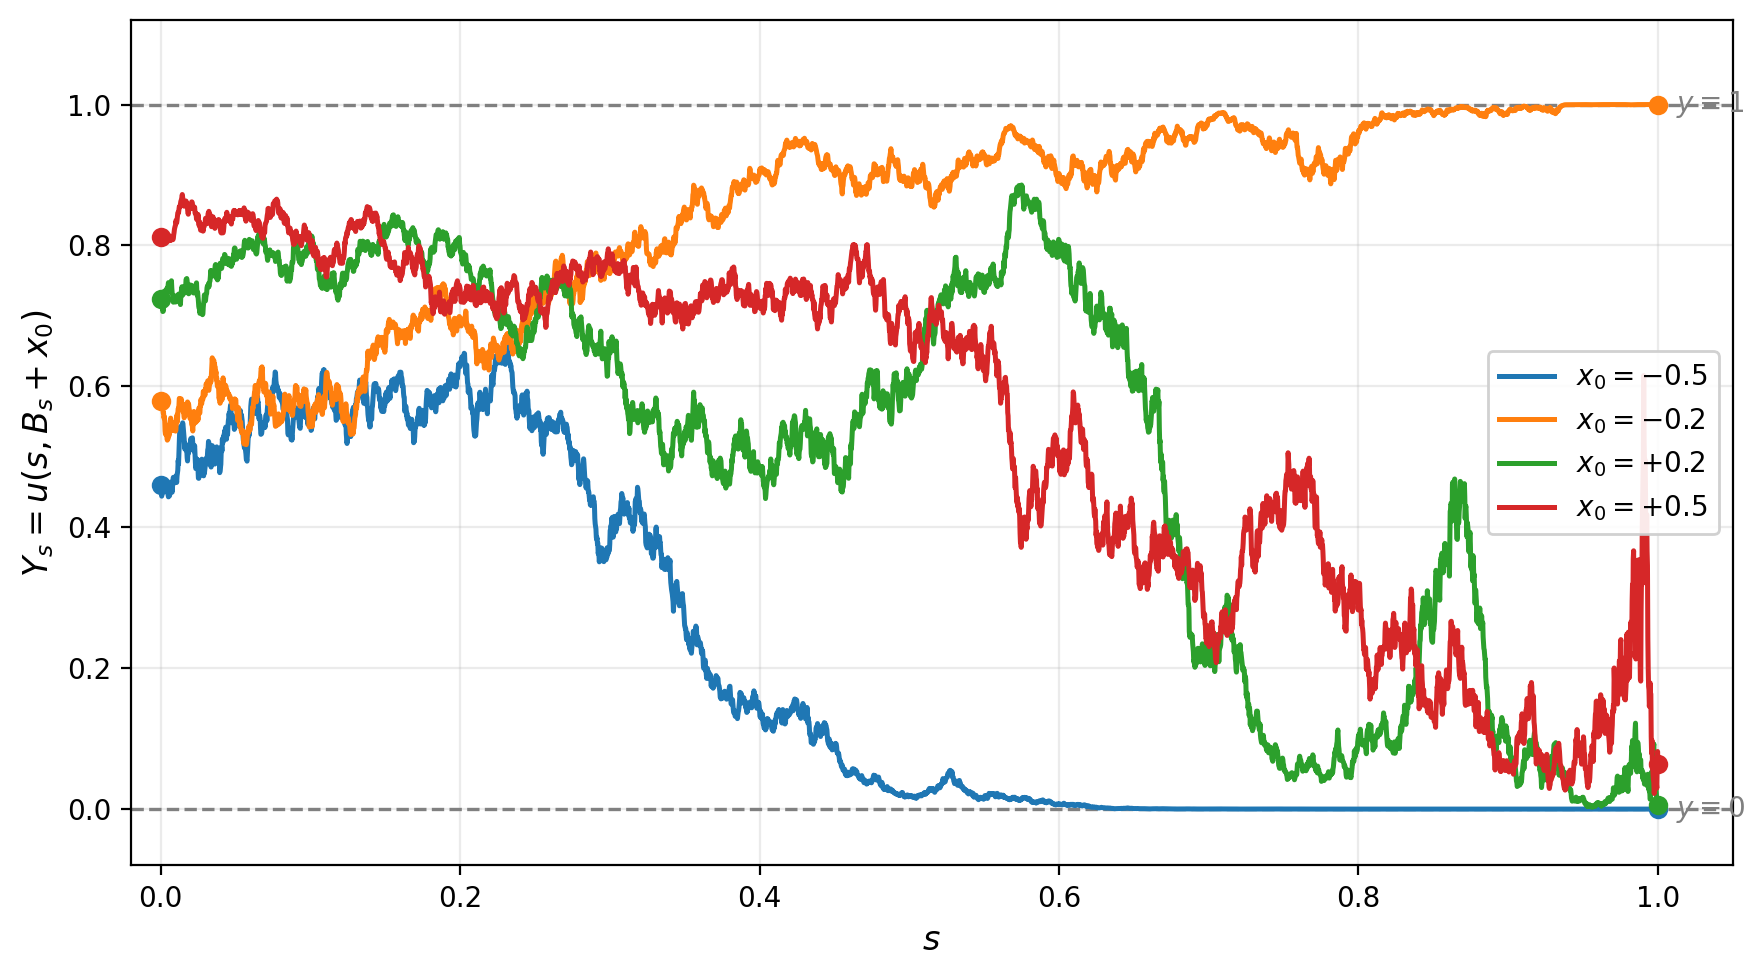
\includegraphics[width=0.9\linewidth]{figures/fig2_fisher_kpp.png}
\caption{Fisher--KPP BSDE 在 $[0, T] = [0, 1]$ 上的四条 $Y$ 轨道，初始位置取 $x_0 \in \{-0.5, -0.2, +0.2, +0.5\}$。我们先在一个细密的 $(t, x)$ 网格上用显式倒推求解 PDE $\partial_t u + \tfrac12 \partial_{xx} u + u(1 - u) = 0$，再抽样布朗路径 $B_s$，绘出 $Y_s = u(s, B_s + x_0)$。所有轨道都停留在 $[0, 1]$ 内：常数 $y \equiv 0$ 与 $y \equiv 1$ 本身分别是终端条件 $\xi = 0$、$\xi = 1$ 的 BSDE 解，比较定理（定理~\ref{thm:comparison}）把每个解夹在它们之间。每条轨道的终端值实现了沿对应布朗路径的指示函数 $\mathbf{1}_{B_T + x_0 > 0}$。}
\label{fig:fisher-kpp}
\end{figure}

\section{应用}

\subsection{随机最优控制与 HJB}

考虑受控扩散
\[
  dX^\alpha_s = b(s, X^\alpha_s, \alpha_s)\, ds + \sigma(s, X^\alpha_s)\, dB_s,
\]
控制 $\alpha$ 取值于紧的作用集 $A \subset \R^k$，且须适应。给定运行成本 $\ell$ 与终端成本 $g$，定义值函数
\[
  V(t, x) := \inf_{\alpha}\, \E\!\left[ \int_t^T \ell(s, X^\alpha_s, \alpha_s)\,ds + g(X^\alpha_T) \,\bigg|\, X^\alpha_t = x \right].
\]
由动态规划原理，$V$ 形式上满足 Hamilton--Jacobi--Bellman 方程
\[
  \partial_t V(t, x) + \inf_{a \in A}\Big\{ b(t, x, a) \cdot \nabla V + \tfrac12\, \mathrm{tr}(\sigma \sigma^{\top}\, \nabla^2 V) + \ell(t, x, a) \Big\} = 0, \quad V(T, x) = g(x).
\]
在 $\sigma$ 不依赖 $a$ 的情形，也就是\emph{漂移控制}，HJB 方程可写成半线性形式。为了与 \eqref{eq:semilinpde} 对齐，可以选取一个参考扩散
\[
  d\bar X_s = b_0(s, \bar X_s)\,ds + \sigma(s, \bar X_s)\,dB_s,
\]
其生成元记为 $\Lc^0$。若 $\sigma$ 可逆，则对应的驱动可写为
\[
  f(t, x, y, z) = \inf_{a \in A}\!\Big\{ \big(b(t, x, a) - b_0(t,x)\big) \cdot \sigma^{-\top}(t, x)\, z + \ell(t, x, a) \Big\}.
\]
若取 $b_0 \equiv 0$，就得到常见的简化公式。若 $\sigma$ 不可逆，则需以 $Z = \sigma^{\top} \nabla V$ 为主要对象，并使用广义 Hamilton 量。对应的 BSDE 在适当条件下给出 $V$ 的概率表示，并为最优反馈控制 $\alpha^*(s, X_s) \in \arg\min_a \{\cdots\}$ 的可测选择提供自然表达。

当 $\sigma$ 也依赖 $a$ 时，问题通常不再是普通的半线性 PDE，而是完全非线性 PDE。此时需要\emph{二阶} BSDE（2BSDE），相关理论可参考 Soner、Touzi 与 Zhang。

\subsection{Deep BSDE：高维 PDE 的深度学习方法}

PDE \eqref{eq:semilinpde} 在高空间维度 $n$ 下是基于网格的求解器力所不及的：每轴 $N$ 个点，存储量为 $\Theta(N^n)$。Han、Jentzen、E 的 \textbf{Deep BSDE} 方法\cite{han-jentzen-e}把求解 PDE 重新表述为单一的全局随机优化问题。将时间离散为 $0 = t_0 < t_1 < \cdots < t_M = T$，$\Delta t = T/M$。参数化：
\begin{itemize}
  \item 初值由一个标量 $\theta_0 \in \R$ 表示（$u(0, x_0)$ 的候选值）；
  \item 空间梯度 $z(t, x) := \sigma^{\top}(t, x)\,\nabla u(t, x)$ 由参数为 $\theta$ 的神经网络 $z^\theta(t, x)$ 给出。
\end{itemize}
从 $x_0$ 出发做 $X$ 的前向 Euler--Maruyama 离散，并沿时间递推
\[
  Y^\theta_{t_{k+1}} = Y^\theta_{t_k} - f\!\big(t_k, X_{t_k}, Y^\theta_{t_k}, z^\theta(t_k, X_{t_k})\big)\, \Delta t + z^\theta(t_k, X_{t_k}) \cdot \Delta B_k,
\]
其中 $Y^\theta_0 = \theta_0$。通过终端不匹配损失
\[
  \mathcal{J}(\theta) := \E\!\left[ \big| g(X_T) - Y^\theta_T \big|^2 \right]
\]
对 $\theta = (\theta_0, \theta_{\rm net})$ 做随机梯度下降训练。在最优处，$\theta_0 \approx u(0, x_0)$，$z^\theta(\cdot, \cdot) \approx \sigma^{\top} \nabla u$。

其数学内容是一个\emph{变分刻画}：$u(0, x_0)$ 是唯一这样的值，使得当 $Y_0 = u(0, x_0)$、$Z$ 为 BSDE 的解时，残差 $g(X_T) - Y_T$ 几乎处处为零。把“几乎处处”换成“$L^2$”即得损失函数，把“BSDE 解 $Z$”换成“最佳神经网络逼近 $z^\theta$”即得算法。$L^2$ 损失与几乎处处相等之间的桥梁，正是 BSDE 唯一性引理的伪装形式。

在实践中，Deep BSDE 方法曾在若干百维基准问题上表现出明显优势，例如 HJB、含违约风险的 Black--Scholes 与 Allen--Cahn 方程。具体误差与运行时间高度依赖网络结构、训练预算、离散化步数和问题本身，因此它更适合被看作高维 PDE 的概率数值框架，而不是一个无条件的精度保证。

\begin{figure}[htbp]
\centering
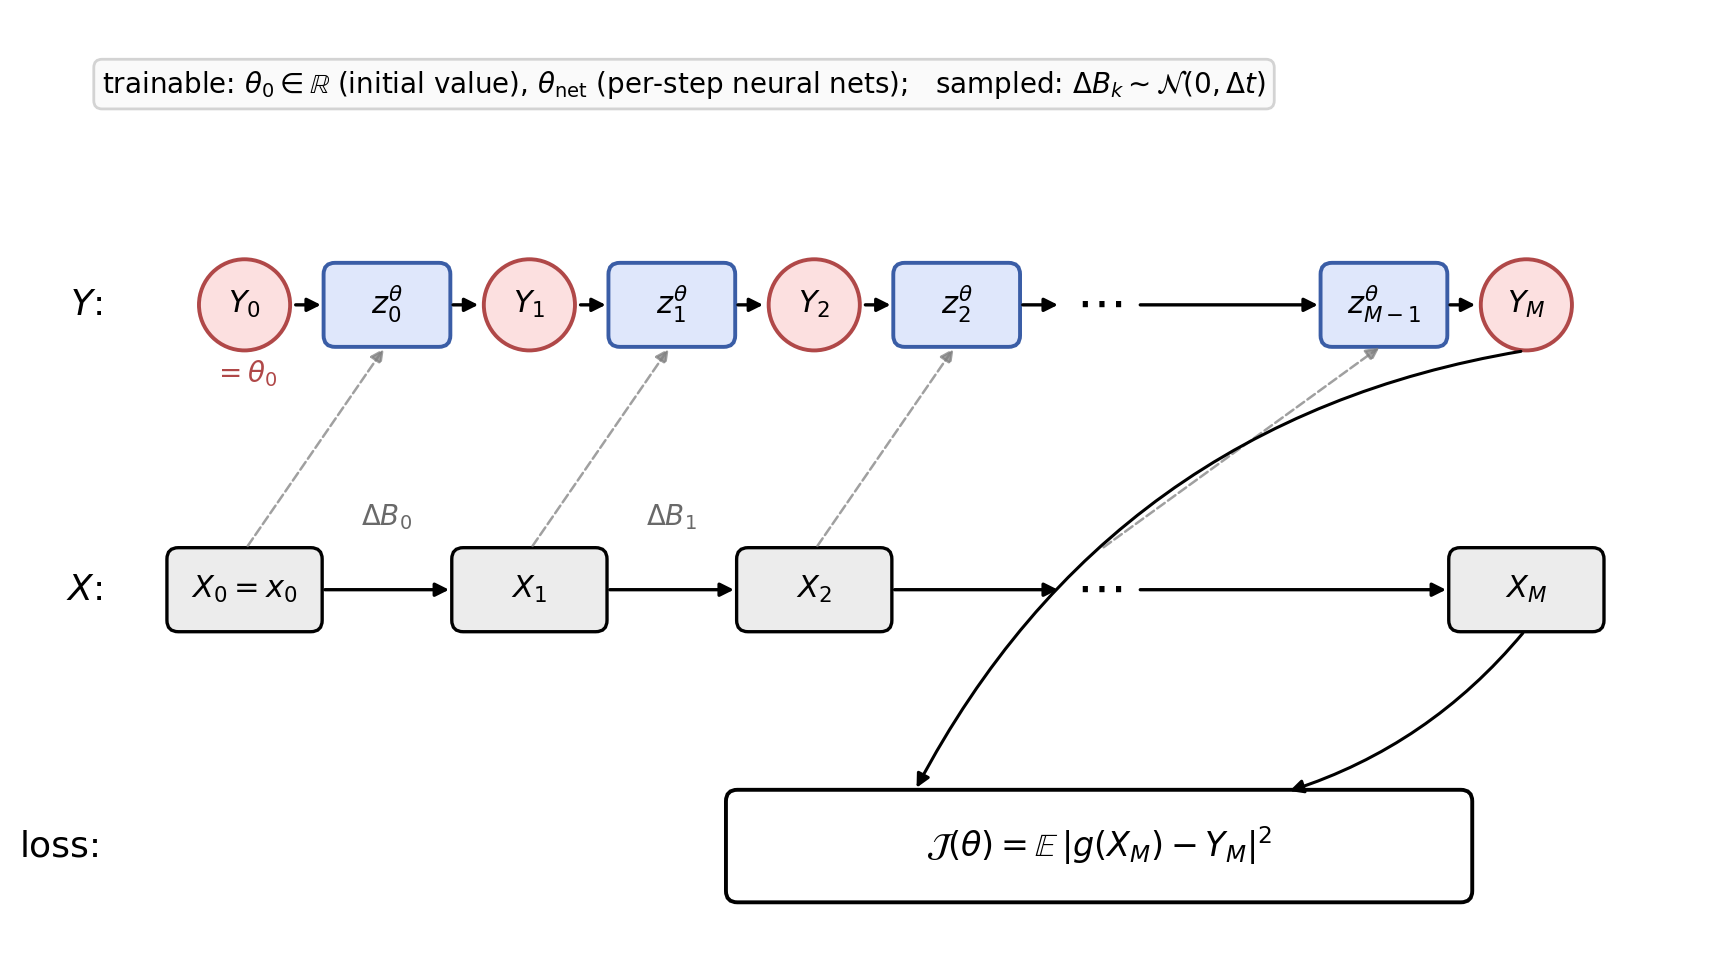
\includegraphics[width=0.95\linewidth]{figures/fig3_deep_bsde.png}
\caption{Deep BSDE 方法的架构。前向链（灰色）是由抽样布朗增量 $\Delta B_k$ 驱动的 $X$ 的 Euler--Maruyama 离散。倒向链（红色与蓝色）从可训练标量 $\theta_0$ 出发，依规则 $Y^\theta_{k+1} = Y^\theta_k - f(t_k, X_k, Y^\theta_k, z^\theta_k)\Delta t + z^\theta_k \cdot \Delta B_k$ \emph{沿时间正向}递推，其中每个 $z^\theta_k$ 是一个小神经网络，将 $X_k$ 映射到 $\sigma^\top(t_k, X_k)\nabla u(t_k, X_k)$。用 SGD 对终端不匹配损失 $\mathcal{J}(\theta)$ 训练，把 $\theta_0$ 推向 $u(0, x_0)$。让这一切起作用的变分刻画，本质上就是定理~\ref{thm:pp} 的唯一性部分。}
\label{fig:deepbsde}
\end{figure}

\section{展望}

本系列下一篇文章可以沿着下列四条线索之一展开。

\paragraph{前向--倒向耦合（FBSDE）。} 若前向系数依赖 $Y$ 或 $Z$，便得到\emph{耦合的}前向--倒向 SDE：
\begin{align*}
  dX_s &= b(s, X_s, Y_s, Z_s)\,ds + \sigma(s, X_s, Y_s, Z_s)\, dB_s, \\
  -dY_s &= f(s, X_s, Y_s, Z_s)\,ds - Z_s\, dB_s, \qquad Y_T = g(X_T).
\end{align*}
这是通过 Pontryagin 极大值原理表达完全耦合随机最优控制的自然语言。其存在性要求单调性条件（Ma--Yong），或短时间假设（Antonelli），或者在 PDE 端有经典解时使用四步法（Ma--Protter--Yong）。

\paragraph{平均场 BSDE。} 让驱动函数依赖边际分布 $\mathcal{L}(Y_s)$，便得到 McKean--Vlasov BSDE，这是平均场博弈的自然语言。对应的 PDE 定义在 $[0, T] \times \R^n \times \mathcal{P}_2(\R^n)$ 上，即所谓的\emph{主方程}（master equation），并联系回 Lions 的 Wasserstein 微积分。

\paragraph{反射型 BSDE 与美式期权。} 反射型 BSDE（El~Karoui--Kapoudjian--Pardoux--Peng--Quenez 1997）为方程加上一个障碍过程 $L = (L_t)$：解是三元组 $(Y, Z, K)$，其中 $K$ 连续非减、$K_0 = 0$，$Y_t \ge L_t$ a.s.，且
\[
  Y_t = \xi + \int_t^T f(s, Y_s, Z_s)\,ds + K_T - K_t - \int_t^T Z_s\, dB_s,
\]
并满足 Skorokhod 条件 $\int_0^T (Y_t - L_t)\,dK_t = 0$。过程 $K$ 把 $Y$ \emph{最少地}向上推，且只在 $Y$ 触及障碍时才推。对应的 PDE 是障碍问题
\[
  \min\!\big\{ -\partial_t u - \Lc u - f(t, x, u, \sigma^{\top}\nabla u),\ u - L \big\} = 0, \qquad u(T, x) = g(x).
\]
若 $f$ 不依赖 $(Y,Z)$，反射型 BSDE 还给出普通最优停时问题的 Snell 包络表示：
\[
  Y_t = \operatorname*{ess\,sup}_{\tau \in [t, T]} \E\!\left[\int_t^\tau f_s\, ds + L_\tau \mathbf{1}_{\tau < T} + \xi \mathbf{1}_{\tau = T} \,\bigg|\, \F_t\right].
\]
若 $f$ 依赖 $(Y,Z)$，上式中的普通条件期望应替换为相应的非线性 $f$-期望。

教科书级的应用是美式期权定价：行权价为 $K$ 的看跌期权取 $L_t = (K - X_t)^+$，折现项 $f \equiv -r y$；提前行权边界正是接触集 $\{Y = L\}$。双障碍（Dynkin 博弈）与二阶变体沿用同一模板。

\paragraph{粗糙路径与粗糙 BSDE。} 若驱动噪声比布朗运动更粗糙（例如 Hurst 参数 $H < 1/2$ 的分数布朗运动），BSDE 背后的 It\^o 微积分就失效了。Lyons 的粗糙路径理论与 Hairer 的正则性结构提供了替代工具；粗糙 BSDE 是活跃的研究领域，Diehl--Friz--Gassiat 的构造是标准参考。

\begin{thebibliography}{9}
\bibitem{pp1990} Pardoux, \'E., Peng, S. \emph{Adapted solution of a backward stochastic differential equation.} Systems Control Lett.\ 14 (1990), 55--61.
\bibitem{el-karoui-quenez} El Karoui, N., Peng, S., Quenez, M.~C. \emph{Backward stochastic differential equations in finance.} Math.\ Finance 7 (1997), 1--71.
\bibitem{han-jentzen-e} Han, J., Jentzen, A., E, W. \emph{Solving high-dimensional partial differential equations using deep learning.} PNAS 115 (2018), 8505--8510.
\bibitem{pardoux-rascanu} Pardoux, \'E., R\u{a}\c{s}canu, A. \emph{Stochastic Differential Equations, Backward SDEs, Partial Differential Equations.} Springer, 2014.
\bibitem{revuz-yor} Revuz, D., Yor, M. \emph{Continuous Martingales and Brownian Motion}, 3rd ed., Springer, 1999.
\end{thebibliography}

\clearpage % 在 CJK* 环境内输出最后一页（页眉含中文标题）
\end{CJK*}
\end{document}
